\documentclass[review]{elsarticle}

\usepackage{lineno,hyperref}
\modulolinenumbers[5]

\journal{Artificial Intelligence class at UFES}

%%%%%%%%%%%%%%%%%%%%%%%
%% Elsevier bibliography styles
%%%%%%%%%%%%%%%%%%%%%%%
%% To change the style, put a % in front of the second line of the current style and
%% remove the % from the second line of the style you would like to use.
%%%%%%%%%%%%%%%%%%%%%%%

%% Numbered
%\bibliographystyle{model1-num-names}

%% Numbered without titles
%\bibliographystyle{model1a-num-names}

%% Harvard
%\bibliographystyle{model2-names.bst}\biboptions{authoryear}

%% Vancouver numbered
%\usepackage{numcompress}\bibliographystyle{model3-num-names}

%% Vancouver name/year
%\usepackage{numcompress}\bibliographystyle{model4-names}\biboptions{authoryear}

%% APA style
%\bibliographystyle{model5-names}\biboptions{authoryear}

%% AMA style
%\usepackage{numcompress}\bibliographystyle{model6-num-names}

%% `Elsevier LaTeX' style
\bibliographystyle{elsarticle-num}
%%%%%%%%%%%%%%%%%%%%%%%

\usepackage{amsmath}
\usepackage{graphics}
\usepackage{float}
\usepackage{cleveref}
\usepackage{listings}
\usepackage{xcolor}
\usepackage{tikz}
\usepackage{pgfplots}

\definecolor{codegreen}{rgb}{0,0.5,0}
\definecolor{codegray}{rgb}{0.5,0.5,0.5}
\definecolor{codepurple}{rgb}{0.58,0,0.82}
\definecolor{backcolour}{rgb}{0.95,0.95,0.95}

\lstdefinestyle{mystyle}{
    backgroundcolor=\color{backcolour},   
    commentstyle=\color{codegreen},
    keywordstyle=\color{magenta},
    numberstyle=\tiny\color{codegray},
    stringstyle=\color{codepurple},
    basicstyle=\ttfamily\footnotesize,
    captionpos=b,
    breaklines=true,
    breakatwhitespace=true,
    % numbers=left,e
    numbersep=5pt,
    tabsize=2,
    showtabs=true,
    showspaces=false,
}
\lstset{style=mystyle}

\begin{document}

\begin{frontmatter}

\title{Experiments with Reinforcement Learning for a Neural Network to Play Dino\\Modality: 2}

%% Group authors per affiliation:
\author{Henrique Coutinho Layber}
\address{Vitória, Espírito Santo, Brazil}

\begin{abstract}

Dino is a simple game where the player controls a dinosaur that has to dodge obstacles. The game is simple enough that a neural network can learn to play it, but it is also complex enough that it is not trivial to play. In this work, we present a neural network that plays the Dino game using Reinforcement Learning. The neural network is trained using Simulated Annealing. The neural network is evaluated by the score it achieves in the game. The results show that it is able to learn to play the game, and that it is able to achieve a higher score than a simple heuristic. It is also able to achieve a higher score than a neural network trained by the professor.

\end{abstract}

\begin{keyword}
Machine learning\sep neural network\sep Reinforcement Learning
\end{keyword}

\end{frontmatter}

\linenumbers

\section{Introduction}

Dino\footnote{Officially available on \url{chrome://dino}, for Chromium browsers only} is a runner game featuring a dinosaur as the player, the goal is to score as high as possible dodging obstacles. The game is very simple, thus a good example of a game that can be played by a neural network. The game is simple enough that a neural network can learn to play it, but it is also complex enough that it is not trivial to play.

One of the ways a neural network can learn to play a game is through Reinforcement Learning. Reinforcement Learning is a type of Machine Learning where an agent learns to behave in an environment, by performing actions and seeing the results of those actions. A common implementation of Reinforcement Learning is with a search heuristic and a classifier. The search heuristic is used to explore the environment (usually neural network's parameters) and the classifier is used to predict the best action to take.

All code for this experiment is available at \url{https://github.com/Henriquelay/AI-classes/tree/main/Trab2/app}

\section{Classifier Description}

For this experiment, the classifier is a neural network specialized in only seeing the immediately next obstacle. It is implemented as a feedforward network with 3 layers: the input layer, the hidden layer, and the output layer. The input layer has 3 neurons: distance to the next obstacle with a predicted physics step built-in, height of the next obstacle, speed of the game. The hidden layer has 2 neurons activated with ReLU and the output layer has 1 neuron activated with sigmoid. If the output is greater than $0.55$, the player jumps, otherwise it ducks.

To figure out how to design the neural network, several trials were made.

\subsection{Input manipulation}

By far the most effective way to impact the classifier was to change the input. As the saying goes, ``\textit{garbage in, garbage out}''. By diminishing the amount of \textit{garbage in}, we can improve the classifier massively with simple changes.

\subsubsection{\texttt{obType}, \texttt{obHeight}}

The only scenario where knowing the type of the object would be useful is when facing a high object you \textit{maybe} could duck under. You can duck under a high enough bird, but have to jump over a cactus regardless of its height. Since there is no other scenario where knowing the type of the object is useful, unless it can be used to differentiate between a high bird (which you can duck under) and a similarly high cactus (which you can't duck under), it is useless.

$$\exists c \exists b [iscactus(c) \land isbird(b) \land height(c) > height(b) \land isduckable(b)] \leftrightarrow obType \; \text{is useful}$$ \label{eq:obType}

However, this scenario is impossible to happen in the implemented game, since birds can only have a height of $\{38, 83, 123\}$, and cactuses can only have a height of $\{38, 58\}$, and the player can only duck under birds of height $83$ or more, there is no cactus higher than a bird that can be ducked under, so differentiating duck-able obstacles is unneeded, since you can always duck under obstacles over $58$ high. Thus, \texttt{obType} is useless.

Also because of this, \texttt{obHeight} can be simplified further with an arbitrary value of $100$ when the players should jump.
\begin{lstlisting}[language=Python]
obHeight = 100 if obHeight < 83 else 0
\end{lstlisting}
This makes learning process much quicker, and the height difference only matters with extremely high level play, where the falling player's hitbox can dodge a low object.

\subsubsection{\texttt{distance}}

\texttt{distance} is actually the distance to the first rendered obstacle. This means that it can assume negative values, which is not ideal for the neural network, since the obstacle is already beaten when \texttt{distance} is negative. To fix this, when \texttt{distance} is negative, it is set to the distance of the next obstacle. Importantly, the \texttt{obHeight} follows.

Also, a simple change to the \texttt{distance} is to make it a prediction of the future, by subtracting the speed of the game from it. This way, the neural network can take actions earlier (like jumping early). This impacts the learning process at higher scores.

\begin{lstlisting}[language=Python]
if distance <= 0:  # if already past, look at next obstacle
    distance = nextObDistance
    obHeight = nextObHeight
distance -= speed
\end{lstlisting}

\section{Metaheuristic Description}

Simulated Annealing is a metaheuristic that is used to find the global optima of a function. It is inspired by the annealing process of metals, where the metal is heated and then slowly cooled down to remove impurities. The algorithm works by starting at a random point and then moving to a new point based on a probability distribution. The probability distribution is based on the difference between the current point and the new point, and the temperature of the system. The temperature is slowly decreased over time, which causes the algorithm to narrow it's search space.

For this implementation, $energy = score$ was used. To avoid noise, the agent plays the game $15$ times and the $avg - std$ of all scores is used as the energy. 

\subsection{Temperature x Cooling Rate}
There are multiple options for how to cool our system. The temperature can be decreased by a constant amount, by a percentage, or by a function. The cooling rate is a metaparameter that determines how fast the temperature decreases. Some well-established functions were experimented with:

\begin{align}
    boltzmann(e) &= \frac{t_0}{\log(e + 1)} \\
    exponential(e) &= t_0 (1 - C_r)^e \\
    geometric(e) &= \frac{t_0}{1 + C_r \cdot e}
\end{align}
\begin{align*}
    \text{where:}\quad 
    e &= \text{epoch}\\
    % t &= \text{temperature}\\
    t_0 &= \text{initial temperature}\\
    C_r &= \text{cooling rate}
\end{align*}

\begin{figure}[H]
    \centering
    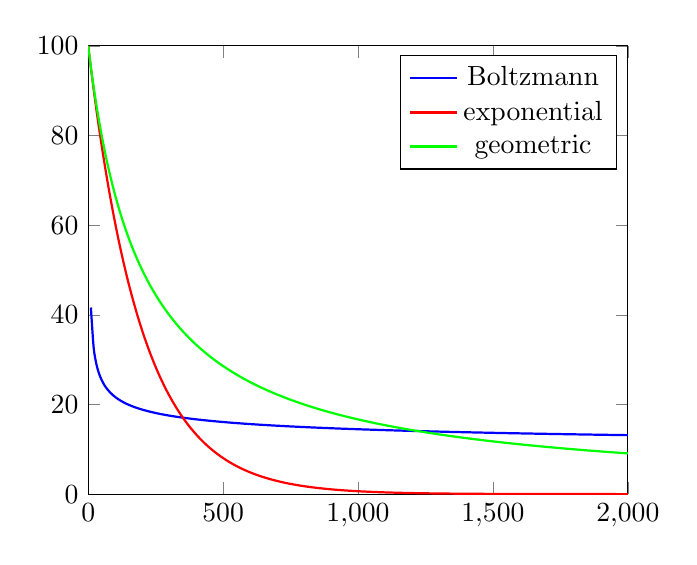
\begin{tikzpicture}
    \begin{axis}[
        xmin = 0, xmax = 2000,
        ymin = 0, ymax = 100]
        \addplot[
            domain = 0:2000,
            samples = 200,
            smooth,
            thick,
            blue,
        ] {100 / ln(x + 1)};
        \addplot[
            domain = 0:2000,
            samples = 200,
            smooth,
            thick,
            red,
        ] {100 * (1 - 0.005)^x};
        \addplot[
            domain = 0:2000,
            samples = 200,
            smooth,
            thick,
            green,
        ] {100 / (1 + 0.005 * x)};
        \legend{
            Boltzmann, 
            exponential,
            geometric
        }
    \end{axis}
    
    \end{tikzpicture}
    \caption{Temperature functions}
    \label{fig:temp}
\end{figure}

For shorter training sessions, it is found that a temperature of $100$ and a cooling rate of $0.005$ with \textit{Boltzmann} works well. For longer training sessions, a starting temperature of $200$ and a cooling rate of $0.003$ \textit{geometric} was used to great effect, although more experimentation is needed for longer training sessions. \textit{exponential} was found to be too aggressive, and the temperature would drop too quickly, narrowing the search space too fast.

\subsection{Perturbation}

The perturbation is the function that generates a new state based on the current state. For this implementation, the perturbation is a random number generated between $0$ and $1$, affected by a damping factor, which takes current temperature into account. The perturbation is then multiplied by temperature summed to the original value. This way, we can scan a huge area initially with big perturbations and decrease the perturbation as the temperature decreases, which makes the algorithm narrows its search space as it goes on.

\begin{lstlisting}[language=Python]
def perturb(weight: float) -> float:
    def perturbation() -> float:
        damper = self.temperature / (self.temperature + 10)
        return np.random.uniform(-damper, damper)

    p = perturbation()
    # print(f"{p=}")
    result = weight + self.temperature * p
    return result
\end{lstlisting}

\section{Results}

Here follows results for $30$ rounds of Dino after a long (around $8$ hours) training session\footnote{The agents did not play the same game simultaneously, because the professor only provided the results of his classifier. So they played different rounds}.

% ours [3311.,3289.25,3622.25,3237.25,3705.75,3155.,3519.25,3728.5,3716.25,3205.75,3327.75,3539.75,3509.5,3680.5,3270.5,3147.75,3607.5,3632.75,3318.,3282.25,2805.5,3224.5,3576.5,3177.,2827.75,3266.75,3069.5,3525.5,3555.,3625.25]
% prof [1214.0,759.5,1164.25,977.25,1201.0,930.0,1427.75,799.5,1006.25,783.5,728.5,419.25,1389.5,730.0,1306.25,675.5,1359.5,1000.25,1284.5,1350.0,751.0,1418.75,1276.5,1645.75,860.0,745.5,1426.25,783.5,1149.75,1482.25,]

\begin{table}[H]
    \centering
    \resizebox{!}{.5\textheight}{%
    \begin{tabular}{|c|c|c|}
        \hline
        &\textbf{Ours} & \textbf{Professor} \\
        \hline
        & $3311.00$ & $1214.00$ \\
        & $3289.25$ & $759.50$ \\
        & $3622.25$ & $1164.25$ \\
        & $3237.25$ & $977.25$ \\
        & $3705.75$ & $1201.00$ \\
        & $3155.00$ & $930.00$ \\
        & $3519.25$ & $1427.75$ \\
        & $3728.50$ & $799.50$ \\
        & $3716.25$ & $1006.25$ \\
        & $3205.75$ & $783.50$ \\
        & $3327.75$ & $728.50$ \\
        & $3539.75$ & $419.25$ \\
        & $3509.50$ & $1389.50$ \\
        & $3680.50$ & $730.00$ \\
        & $3270.50$ & $1306.25$ \\
        & $3147.75$ & $675.50$ \\
        & $3607.50$ & $1359.50$ \\
        & $3632.75$ & $1000.25$ \\
        & $3318.00$ & $1284.50$ \\
        & $3282.25$ & $1350.00$ \\
        & $2805.50$ & $751.00$ \\
        & $3224.50$ & $1418.75$ \\
        & $3576.50$ & $1276.50$ \\
        & $3177.00$ & $1645.75$ \\
        & $2827.75$ & $860.00$ \\
        & $3266.75$ & $745.50$ \\
        & $3069.50$ & $1426.25$ \\
        & $3525.50$ & $783.50$ \\
        & $3555.00$ & $1149.75$ \\
        & $3625.25$ & $1482.25$ \\
        \hline
        \textbf{Mean} & $3381.99$ & $1068.18$ \\
        \textbf{Std} & $246.54$ & $304.04$ \\
        \textbf{t-test} & \multicolumn{2}{|c|}{$2.00e-38$} \\
        \textbf{Wilcoxon} & \multicolumn{2}{|c|}{$1.86e-09$} \\
        \hline
    \end{tabular}
    }
    \caption{Score comparison}
    \label{tab:scores}
\end{table}

\begin{figure}[H]
    \centering
    \includegraphics[width=.7\linewidth]{energy_epoch.pdf}
    \caption{Energy (score) over epochs}
    \label{fig:energy}
\end{figure}

Here we include a third agent (\textit{simplest}), which is included with the game's implementation. The agent plays the same round as our agent, but it is not a neural network, it is a simple heuristic that jumps when the obstacle is close.

\begin{figure}[H]
    \centering
    \includegraphics[width=.7\linewidth]{agent_comparison.pdf}
    \caption{Score over epochs}
    \label{fig:score_comparison}
\end{figure}

\section{Conclusions}
\subsection{General Result Analysis}

Aside from the initial burst to $\approx 1200$ when the agent learns to basic jump and duck, we can see that from epoch $152$ to $154$ there is another huge jump in score. This is when the agent learns to jump earlier at high speeds. Jumping late at high speeds is a common way to lose the game, since it's likely that the player can't jump the following obstacle due to landing on it, or not having enough time to get high enough.

We can see that our agent is statistically different from the professor's agent, with a $p$-value of $2.00e-38$ for the t-test and $1.86e-09$ for the Wilcoxon test.

\subsection{Contribution}

The main contribution of this work is the implementation of a neural network to play the Dino game, using Reinforcement Learning. \\
The single biggest improvement was the input manipulation, which made the learning process much quicker. In special, the \texttt{obHeight} manipulation was the most impactful, since it made the learning process much quicker and the network design simpler. \\
The second-biggest improvement were the cooling functions experiments, which made the learning process more stable and resilient to noise.

\subsection{Future Work}

The main limitation of this work is the lack of a proper evaluation of the neural network. The neural network was only evaluated by the score it achieved, but it would be interesting to evaluate it in other ways, such as the number of jumps it made, the number of obstacles it dodged, and the number of times it died. It would also be interesting to evaluate the neural network on other games, to see how well it generalizes.

% \bibliography{mybibfile}

\end{document}
